\begin{figure}[H]
\centering
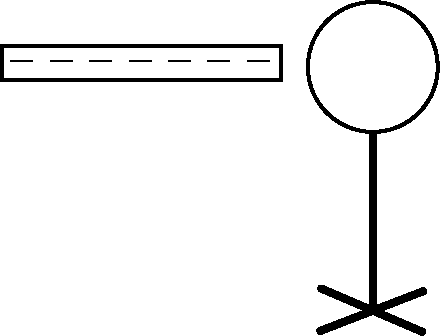
\includegraphics[scale=0.25]{images/img-007-021.png}
\end{figure}

% Multiple Choice Question 10
\begin{questions}\setcounter{question}{9}\question
A spherical conductor is on an insulating stand, as shown in the figure above. A negatively charged rod is brought close to the sphere but does not touch the sphere. Which of the following describes the resulting charge on the sphere?

\begin{choices}
\choice Positive
\choice Negative
\choice No net charge, but the sphere is polarized with positive charge on the left side.
\choice No net charge, but the sphere is polarized with negative charge on the left side.
\choice No net charge and no polarization
\end{choices}\end{questions}

